\documentclass{scrartcl}

\usepackage{amssymb}
\usepackage{amsmath}
\usepackage{tikz}
\usetikzlibrary{decorations.pathreplacing}	%for brackets (fig. 1)
\usetikzlibrary{calc}						%for centerarc (fig. 2)

%Kwan, C. (2013). ``Business Cycle in China since the Lehman Crisis: Interaction among Macroeconomic Policy, Economic Growth and Inflation.'' China & World Economy 21(5), pp. 1-19 -- fig. 4 \& 5

\def\centerarc[#1](#2)(#3:#4:#5)% Syntax: [draw options] (center) (initial angle:final angle:radius)
{ \draw[#1] ($(#2)+({#5*cos(#3)},{#5*sin(#3)})$) arc (#3:#4:#5); }

\begin{document}
	
	\begin{figure}
		\centering
		\vspace*{-0.5in}	%just for spacing; otherwise, goes to middle of page
	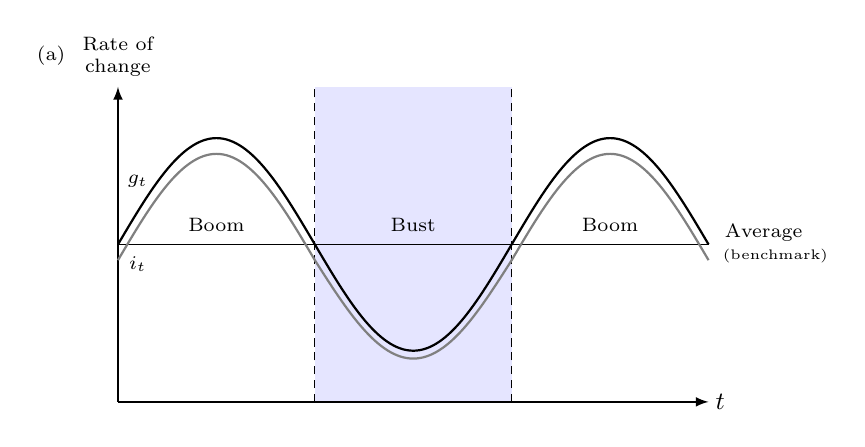
\begin{tikzpicture}
	%axis
	\fill[blue!10!white] (2.5,0) rectangle (5,4);	%middle shading
	\draw[->,>=latex,semithick] (0,0)--(0,4);		%y-axis
	\draw[->,>=latex,semithick] (0,0)--(7.5,0);		%x-axis
	\node at (-.85,4.4)	{{\scriptsize (a)}};
	\node at (0,4.55) 	{{\scriptsize Rate of}};
	\node at (0,4.25) 	{{\scriptsize change}};
	\node at (7.65,0)   {{\small $t$}};
	
	%lines
	\draw[semithick] (0,2)--(7.5,2);		%benchmark
	\draw[densely dashed] (2.5,0)--(2.5,4);	%boom #1 | bust
	\draw[densely dashed] (5,0)--(5,4);		%bust | boom #2
	
	%business cycles
	\draw[thick] (0,2) sin (1.25,3.35) cos (2.5,2) sin (3.75,0.65) cos (5,2) sin (6.25,3.35) cos (7.5,2); %g
	\draw[thick,gray](0,1.8) sin (1.25,3.15) cos (2.5,1.8) sin (3.75,0.55) cos (5,1.8) sin (6.25,3.15) cos (7.5,1.8); %i
	\node at (0.25,2.80) {{\scriptsize $g_t$}};
	\node at (0.25,1.75) {{\scriptsize $i_t$}};
	
	%labels
	\node at (1.25,2.25) {{\scriptsize Boom}};
	\node at (3.75,2.25) {{\scriptsize Bust}};
	\node at (6.25,2.25) {{\scriptsize Boom}};
	\node at (8.2,2.15)	 {{\scriptsize Average}};
	\node at (8.35,1.85) {{\tiny (benchmark)}};
	
	%\draw[help lines] (0,0) grid (6,4);
	\end{tikzpicture}
	
	
	%\vspace{0.25cm}
	
	
	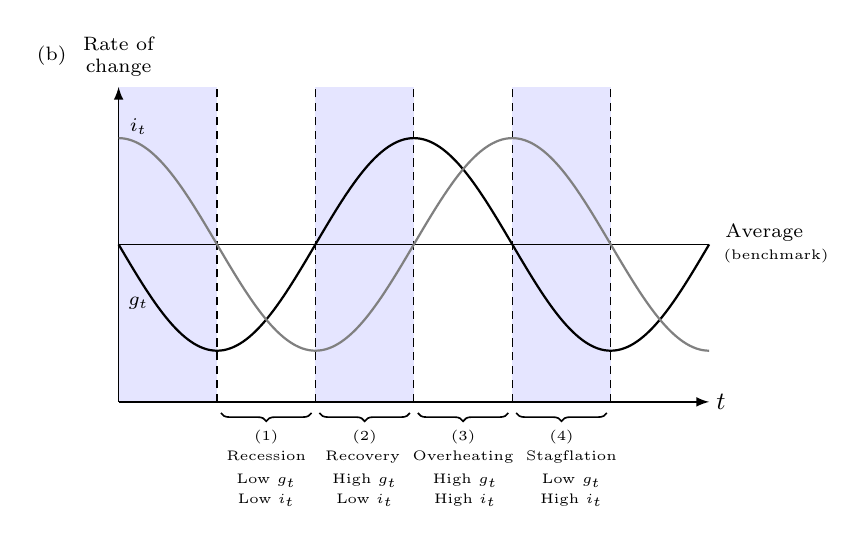
\begin{tikzpicture}
	%shading
	\fill[blue!10!white] (0,0) rectangle (1.25,4);	 %start period
	\fill[blue!10!white] (2.5,0) rectangle (3.75,4); %recovery
	\fill[blue!10!white] (5,0) rectangle (6.25,4);	 %stagflation
	
	%axis
	\draw[->,>=latex,semithick] (0,0)--(0,4);		%y-axis
	\draw[->,>=latex,semithick] (0,0)--(7.5,0);		%x-axis
	\node at (-.85,4.4)	{{\scriptsize (b)}};
	\node at (0,4.55) 	{{\scriptsize Rate of}};
	\node at (0,4.25) 	{{\scriptsize change}};
	\node at (7.65,0)   {{\small $t$}};
	\node at (8.2,2.15)	{{\scriptsize Average}};
	\node at (8.35,1.85){{\tiny (benchmark)}};
	
	%lines
	\draw[semithick] (0,2)--(7.5,2);			%benchmark
	\draw[densely dashed] (1.25,0)--(1.25,4);	%start | recession
	\draw[densely dashed] (2.5,0)--(2.5,4);		%recession | recovery
	\draw[densely dashed] (3.75,0)--(3.75,4);	%recovery | overheating
	\draw[densely dashed] (5,0)--(5,4);			%overheating | stagflation
	\draw[densely dashed] (6.25,0)--(6.25,4);	%stagflation | end
	
	%business cycles
	\draw[thick] (0,2) sin (1.25,0.65) cos (2.5,2) sin (3.75,3.35) cos (5,2) sin (6.25,0.65) cos (7.5,2); %g
	\draw[thick,gray] (0,3.35)cos(1.25,2)sin(2.5,0.65) cos (3.75,2) sin (5,3.35) cos (6.25,2) sin (7.5,0.65); %i
	\node at (0.25,3.5)  {{\scriptsize $i_t$}};
	\node at (0.25,1.25) {{\scriptsize $g_t$}};
	
	%lower labels
	\draw[decorate,decoration={brace,amplitude=3pt},yshift=-4pt,semithick] (2.45,0)--(1.3,0);
	\draw[decorate,decoration={brace,amplitude=3pt},yshift=-4pt,semithick] (3.7,0)--(2.55,0);
	\draw[decorate,decoration={brace,amplitude=3pt},yshift=-4pt,semithick] (4.95,0)--(3.8,0);
	\draw[decorate,decoration={brace,amplitude=3pt},yshift=-4pt,semithick] (6.2,0)--(5.05,0);
	%
	\node at (1.875,-.68) {\tiny Recession};	\node at (1.875,-.45) {\tiny (1)};
	\node at (3.100,-.7)  {\tiny Recovery};		\node at (3.125,-.45) {\tiny (2)};
	\node at (4.375,-.7)  {\tiny Overheating};	\node at (4.375,-.45) {\tiny (3)};
	\node at (5.75,-.7)   {\tiny Stagflation};	\node at (5.625,-.45) {\tiny (4)};
	%
	\node at (1.875,-1) {\tiny Low $g_t$};		\node at (1.875,-1.25) {\tiny Low $i_t$};
	\node at (3.125,-1) {\tiny High $g_t$};		\node at (3.125,-1.25) {\tiny Low $i_t$};
	\node at (4.4,-1)	{\tiny High $g_t$};		\node at (4.4,-1.25)   {\tiny High $i_t$};
	\node at (5.75,-1)  {\tiny Low $g_t$};		\node at (5.75,-1.25)  {\tiny High $i_t$};
	%\draw[help lines] (0,0) grid (6,4);
	\end{tikzpicture}
		\caption{Business cycle phases: (a) without time lags; (b) with time lags}
	\end{figure}
	
	
	
	\begin{figure}
		\centering
		\vspace{1cm}		%just for spacing
	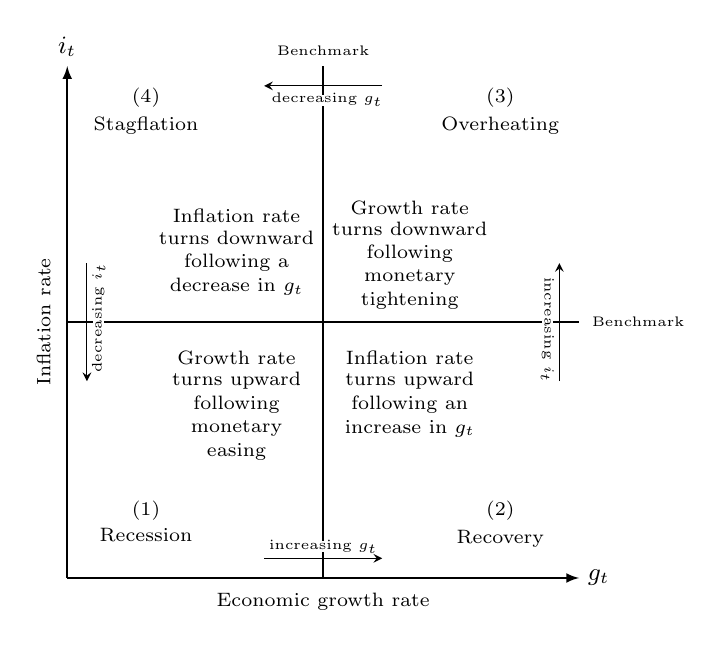
\begin{tikzpicture}
	%axis
	\draw[->,>=latex,semithick] (0,0)--(0,6.5);		%y-axis
	\draw[->,>=latex,semithick] (0,0)--(6.5,0);		%x-axis
	\draw[semithick] (0,3.25)--(6.5,3.25);			%horizontal benchmark
	\draw[semithick] (3.25,0)--(3.25,6.5);			%vertical benchmark
	\node at (6.75,0)   {{\small $g_t$}};
	\node at (0,6.75)   {{\small $i_t$}};
	
	%quadrant labels
	\node at (1,0.55)	{\scriptsize Recession};		\node at (1,0.85)	{\scriptsize (1)};
	\node at (5.5,0.5) 	{\scriptsize Recovery};			\node at (5.5,0.85)	{\scriptsize (2)};
	\node at (5.5,5.75) {\scriptsize Overheating};		\node at (5.5,6.1)	{\scriptsize (3)};
	\node at (1,5.75) 	{\scriptsize Stagflation};		\node at (1,6.1)	{\scriptsize (4)};
	
	%labels in circle
	\node at (2.15,4.6) {\scriptsize Inflation rate};
	\node at (2.15,4.32){\scriptsize turns downward};
	\node at (2.15,4.0) {\scriptsize following a};
	\node at (2.15,3.7) {\scriptsize decrease in $g_t$};
	%
	\node at (2.15,2.8) {\scriptsize Growth rate};
	\node at (2.15,2.5) {\scriptsize turns upward};
	\node at (2.15,2.2) {\scriptsize following};
	\node at (2.15,1.9) {\scriptsize monetary};
	\node at (2.15,1.6) {\scriptsize easing};
	%
	\node at (4.35,4.70) {\scriptsize Growth rate};
	\node at (4.35,4.44) {\scriptsize turns downward};
	\node at (4.35,4.12) {\scriptsize following};
	\node at (4.35,3.82) {\scriptsize monetary};
	\node at (4.35,3.52) {\scriptsize tightening};
	%
	\node at (4.35,2.8) {\scriptsize Inflation rate};
	\node at (4.35,2.5) {\scriptsize turns upward};
	\node at (4.35,2.2) {\scriptsize following an};
	\node at (4.35,1.9) {\scriptsize increase in $g_t$};
	
	%circular arrows
	%\draw[ultra thick,red] (3.25,3.25) circle (2.5cm);
	\centerarc[->,>=stealth,very thick](3.25,3.25)(45:134.5:2.5)
	\centerarc[->,>=stealth,very thick](3.25,3.25)(135:224.5:2.5)
	\centerarc[->,>=stealth,very thick](3.25,3.25)(225:314.5:2.5)
	\centerarc[->,>=stealth,very thick](3.25,3.25)(-45:44.5:2.5)
	
	%labels
	\node at (3.25,6.70) {\tiny Benchmark};		%top
	\node at (7.25,3.25) {\tiny Benchmark};		%side
	\node at (-.3,3.25) {\rotatebox{90}{\scriptsize{Inflation rate}}};
	\node at (3.25,-.3) {\scriptsize{Economic growth rate}};
	
	%arrows between quadrants
	\draw[white,line width=4] (4,6.07)--(2.5,6.07);		%manual fill
	\node at (3.3,6.07) {{\tiny decreasing $g_t$}};		%top
	\draw[->,>=stealth] (4,6.25)--(2.5,6.25);
	%
	\draw[white,line width=4] (2.5,0.4)--(4,0.4);		%manual fill
	\node at (3.25,0.4) {{\tiny increasing $g_t$}};		%bottom
	\draw[->,>=stealth] (2.5,0.25)--(4,0.25);
	%
	\draw[white,line width=4] (6.1,2.5)--(6.1,4);		%manual fill
	\node at (6.1,3.15) {\rotatebox{270}{\tiny increasing $i_t$}};	%right
	\draw[->,>=stealth] (6.25,2.5)--(6.25,4);
	%
	\draw[white,line width=4] (0.4,4)--(0.4,2.5);		%manual fill
	\node at (0.4,3.3) {\rotatebox{90}{\tiny decreasing $i_t$}};	%left
	\draw[->,>=stealth] (0.25,4)--(0.25,2.5);
	
	\end{tikzpicture}
		\caption{Business cycles: interaction between growth \& inflation}
	\end{figure}
\end{document}